\documentclass[table]{beamer}
\mode<presentation>
\usetheme{Berlin}
\usecolortheme{beaver}
\usepackage{multirow}

%%%
% TITLE PREAMBLE
\title[Intro to Bioinformatics] % (optional, only for long titles)
{An Introduction to Bioinformatics Tools}
\subtitle{Basics of Robust and Repeatable Data Analysis}
\author[Pritchard, Cock] % (optional, for multiple authors)
{Leighton~Pritchard \and Peter~Cock}
\institute[The James Hutton Institute] % (optional)
{
  Information and Computational Sciences\\
  The James Hutton Institute
}
\date[May 2014] % (optional)
{Bioinformatics Training, 29$^{th}$ May 2014}
\subject{Bioinformatics}

%%%
% TOC
% Show table of contents, with current section highlighted,
% at the start of each section
\AtBeginSection[]
{
  \begin{frame}
    \frametitle{Table of Contents}
    \tableofcontents[currentsection]
  \end{frame}
}


%%%
% START DOCUMENT
\begin{document}

  \frame[plain]{\titlepage}

 %%%
 % SECTION: Introduction
  \section{Introduction}
  \begin{frame}
    \frametitle{Introduction}
    \framesubtitle{So you want to be a computational biologist?}
    \begin{itemize}
      \item Biology using computational and mathematical tools
      \item Bioinformatics/computational biology is a discipline within biology
      \item Loman \& Watson (2013) \url{http://dx.doi.org/10.1038/nbt.2740}
	  \item \url{http://biomickwatson.wordpress.com/2014/03/10/the-only-core-competency-youre-ever-going-to-need/}
	  \item Welch \textit{et al.} (2014) \url{http://dx.doi.org/10.1371/journal.pcbi.1003496}
	\end{itemize}
  \end{frame}

  \begin{frame}
    \frametitle{Introduction}
    \framesubtitle{Uncomfortable truths}
    \begin{itemize}
      \item This one-day course will not make you a bioinformatician
      \item We will introduce some useful tools and concepts
      \item Most bioinformatics is problem-solving
      \item The best way to learn is to do ("I don't know how to do this yet, but I will find out.")
      % Links to http://biomickwatson.wordpress.com/2013/08/06/bioinformatics-is-not-something-you-are-taught-its-a-way-of-life/
      \item \url{http://bit.ly/Rq0D61}
    \end{itemize}
  \end{frame}

  \begin{frame}
    \frametitle{Introduction}
    \framesubtitle{What it takes to be a bioinformatician}
    \begin{columns}[t]
	  \begin{column}{5cm}
        \begin{itemize}
          \item Patience (problem-solving)
          \item Suspicion (statistics)
          \item Biological knowledge
          \item Social skills (no-one knows everything: ask!)
	    \end{itemize}
	  \end{column}
	  \begin{column}{5cm}
	    \begin{itemize}
	      \item Self-confidence (challenge results)
	      \item Core domain skills: biology, computer science, statistics
	      \item Deliver results (qualified, honest)
	      \item Lots of practice
		\end{itemize}
	  \end{column}
	\end{columns}
	\begin{itemize}
	  % Link goes to http://biomickwatson.wordpress.com/2013/03/18/the-alternative-what-it-takes-to-be-a-bioinformatician/
	  \item \url{http://bit.ly/1jDuQsO}
	  \item \url{http://science.slashdot.org/comments.pl?sid=3161217&cid=41542125}
	\end{itemize}
  \end{frame}


   \begin{frame}
     \frametitle{Where to get more advice?}
     \begin{itemize}
	   \item Ask us (we do this a lot)
	   \item BioStars (\url{https://www.biostars.org})
	   \item SeqAnswers (\url{http://seqanswers.com/})
	   \item \textit{PLoS Comp Biol} collections (\url{http://www.ploscollections.org/static/pcbiCollections})
	\end{itemize}
	
\includegraphics[width=.2\textwidth]{images/gibas_book}
	
\includegraphics[width=.2\textwidth]{images/buffalo_book}
	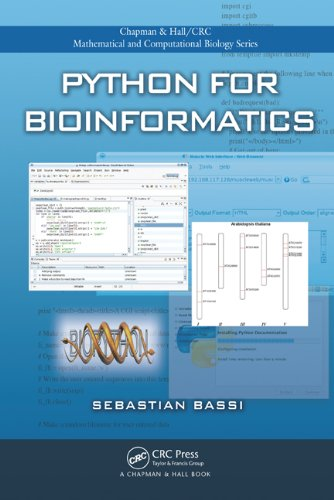
\includegraphics[width=.2\textwidth]{images/bassi_book}
	
\includegraphics[width=.2\textwidth]{images/korf_book}
	
\includegraphics[width=.2\textwidth]{images/model_book}
   \end{frame}

 %%%
 % SECTION: Recording your work
   \section{Recording Your Work}
   
   % SUBSECTION: justification
   \subsection{Why and How?}
   \begin{frame}
     \frametitle{Why Do It?}
     \begin{itemize}
	   \item Doing bioinformatics is doing science: keep a lab book!
	   \item Reproducibility is key! (e.g. Baggerly \& Coombes (2009) \url{http://arxiv.org/pdf/1010.1092.pdf})
	   \item \textit{You won't remember} multiple files, analysis details, etc.
	   \item See: Noble (2009) \url{http://dx.doi.org/10.1371/journal.pcbi.1000424}
	\end{itemize}
	
\includegraphics[width=.7\textwidth]{images/noble_2009_head}
   \end{frame}
   
   \begin{frame}
     \frametitle{How To Do It? I}
     \begin{itemize}
	   \item There is no one correct way, but$\ldots$
	   \item Think about data/docs/project structure \textit{before} you start
	\end{itemize}
    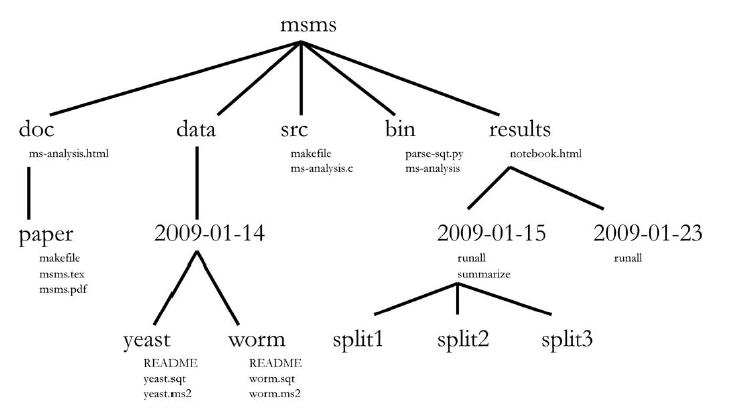
\includegraphics[width=.7\textwidth]{images/project_structure}
   \end{frame}

   \begin{frame}
     \frametitle{How To Do It? II}
     \begin{itemize}
	   \item Use plain text where possible
	   \item Use version control
	   \item Keep backups
	   \item Different tools suit different purposes: code \textit{vs.} data \textit{vs.} analysis \textit{vs.} $\ldots$
	\end{itemize}
   \end{frame}
   
   
   % SUBSECTION: useful tools
   \subsection{Useful Tools}
   \begin{frame}
     \frametitle{Plain Text Files}
     \begin{itemize}
       \item \texttt{README.txt}/\texttt{README.md} in each directory/folder
       \item Plain text is always human-readable
       \item Markdown (\url{https://daringfireball.net/projects/markdown/basics})
       \item RST (\url{http://docutils.sourceforge.net/docs/ref/rst/restructuredtext.html})
     \end{itemize}
    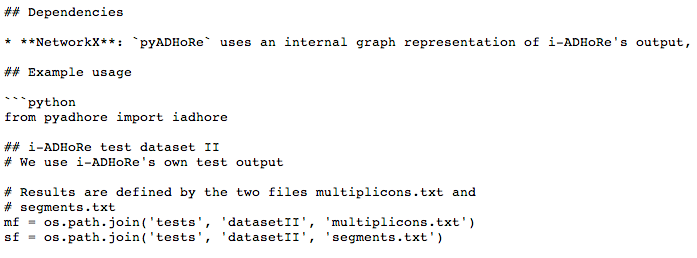
\includegraphics[width=.4\textwidth]{images/markdown_before}
	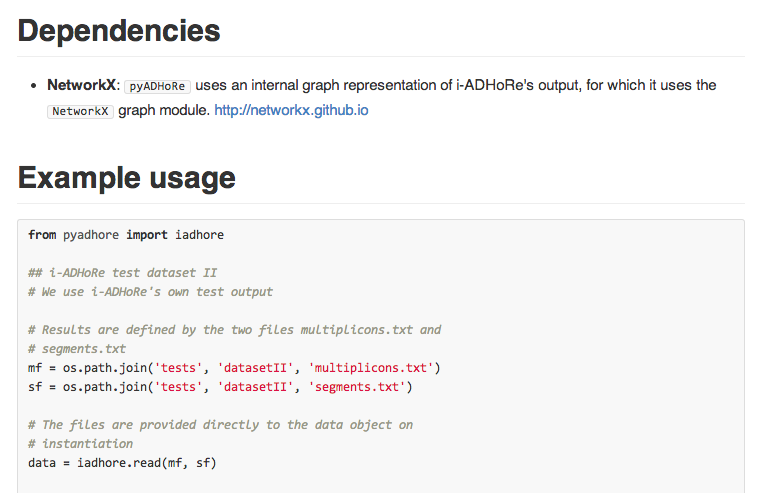
\includegraphics[width=.4\textwidth]{images/markdown_after}
   \end{frame}
   
   \begin{frame}
     \frametitle{\texttt{script}}
     \begin{itemize}
       \item use \texttt{man script} at your terminal
       \item Writes your terminal activity to a plain text file
       \item Saves effort copy/pasting and typing commands into a lab book, as you go
       \item Easy to use with other tools 
     \end{itemize}
   \end{frame}   
   
   \begin{frame}
     \frametitle{\LaTeX}
     \begin{itemize}
       \item Powerful, versatile typesetting system
       \item Similar to markup/markdown
       \item Great for mathematical/computing work
     \end{itemize}
    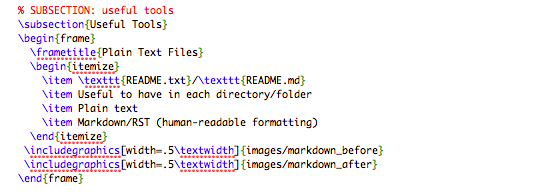
\includegraphics[width=.35\textwidth]{images/latex_before}
	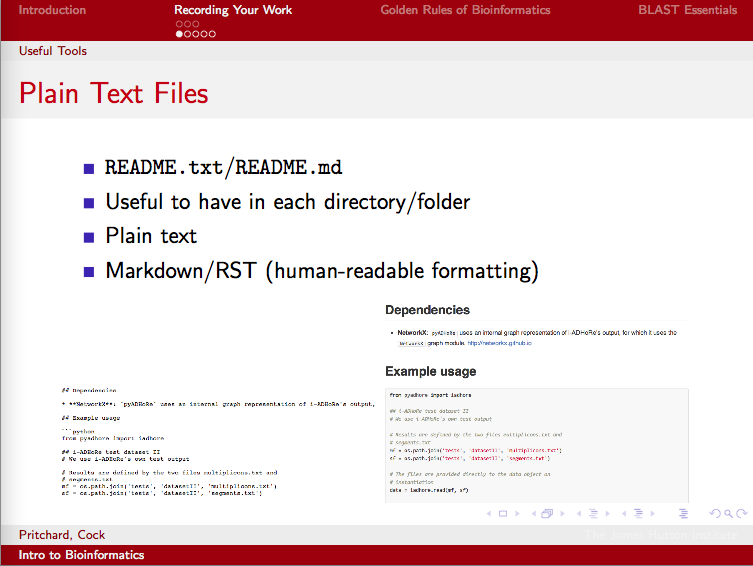
\includegraphics[width=.35\textwidth]{images/latex_after}     
   \end{frame}
   
   \begin{frame}
     \frametitle{MediaWiki}
     \begin{itemize}
       \item Useful for shared projects/data
       \item Automatic version control and attribution
       \item Many local instances at JHI (ask around)
     \end{itemize}
    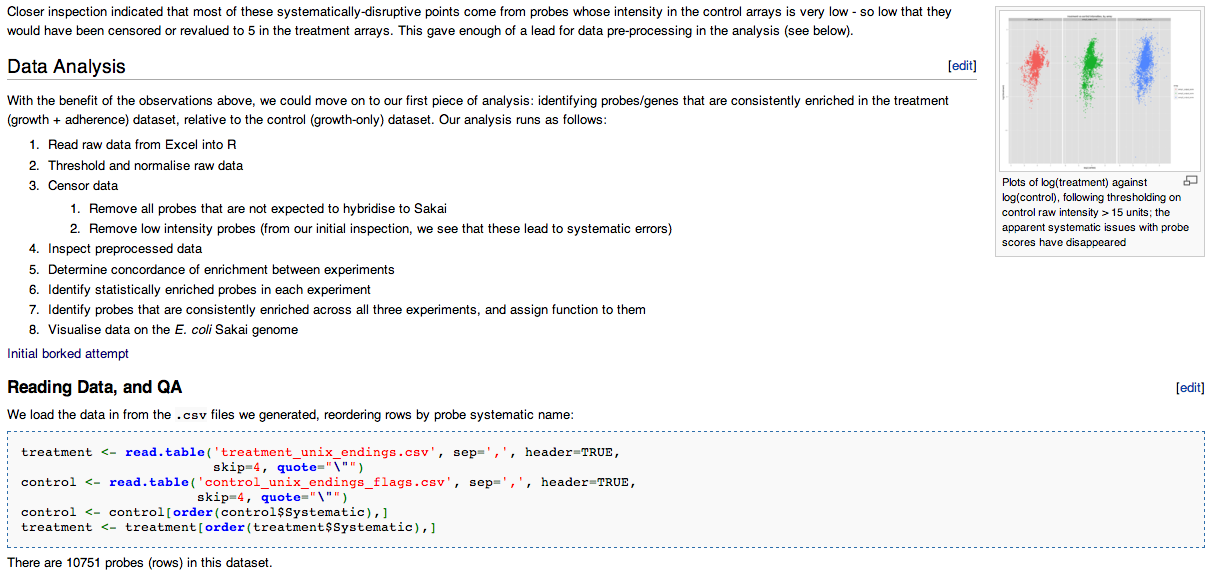
\includegraphics[width=.4\textwidth]{images/mediawiki_after}
	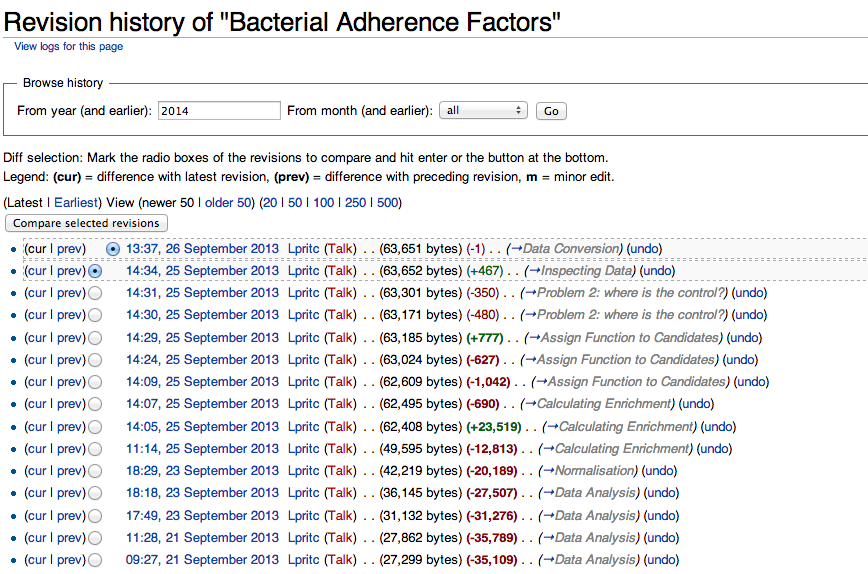
\includegraphics[width=.4\textwidth]{images/mediawiki_version_control}     
   \end{frame}
   
   \begin{frame}
     \frametitle{A language notebook}
     \begin{itemize}
       \item e.g. \texttt{iPython Notebook}, \texttt{Mathematica}, \texttt{MatLab} cells
       \item Integrates live code and analysis with lab-book
     \end{itemize}
    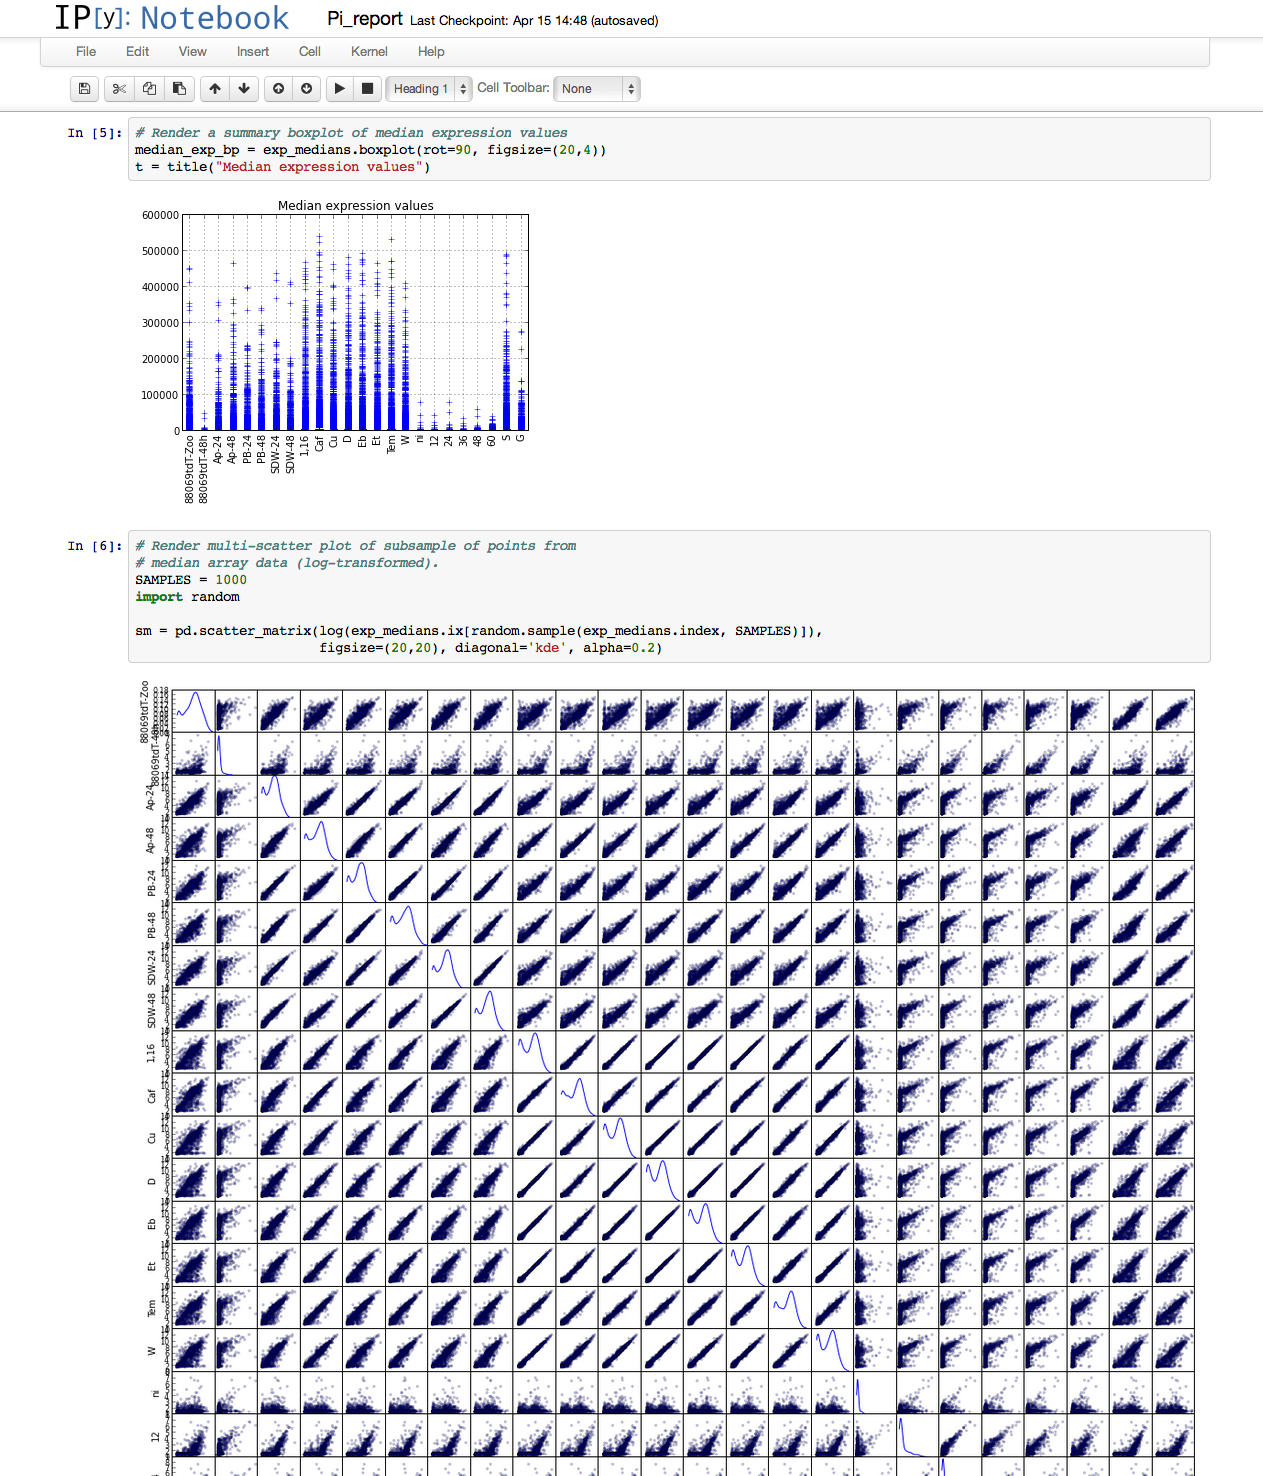
\includegraphics[width=.5\textwidth]{images/ipython_notebook}     
   \end{frame}


 %%%
 % SECTION: The Golden Rules of Bioinformatics
  \section{Golden Rules of Bioinformatics}
  
  \subsection{Rule 1}
  \begin{frame}
    \frametitle{Exercise 1}
    \framesubtitle{Subgroups}
    \begin{itemize}
      \item You are in group A, B, C or D - this decides your dataset: \\
      \texttt{expnA.tab}, \texttt{expnB.tab}, \texttt{expnC.tab}, \texttt{expnD.tab}
      \item You will use \texttt{R} at the command-line to analyse your data
    \end{itemize}
  \end{frame}
  
  \begin{frame}
    \frametitle{Exercise 1}
    \framesubtitle{The biological question}
    \begin{itemize}
      \item Your dataset \texttt{expn?.tab} describes (log) expression data
      \item Two genes: \texttt{gene1} and \texttt{gene2}
      \item Eleven time points (including control)
      \item Q: Are \texttt{gene1} and \texttt{gene2} genes coregulated?
      \item How do we answer this question?
    \end{itemize}
  \end{frame}  

  \begin{frame}
    \frametitle{Exercise 1}
    \framesubtitle{Reformulating the question}
    \begin{itemize}
      \item Q: Are \texttt{gene1} and \texttt{gene2} genes coregulated?
      \item A: We cannot determine this from expression data alone
      \item Reformulate the question:
      \item NewQ: Are \texttt{gene1} and \texttt{gene2} genes coexpressed? \\
            (are expressions \texttt{gene1} $\propto$ \texttt{gene2})
      \item How do we answer this new question?
    \end{itemize}
  \end{frame}

  \begin{frame}
    \frametitle{Exercise 1}
    \framesubtitle{Starting the analysis}
    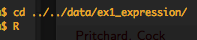
\includegraphics[width=.5\textwidth]{images/ex1_screenshot_a}
  \end{frame}

  \begin{frame}
    \frametitle{Exercise 1}
    \framesubtitle{Starting the analysis}
    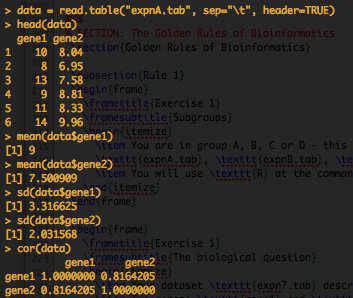
\includegraphics[width=.5\textwidth]{images/ex1_screenshot_b}
  \end{frame}

  \begin{frame}
    \frametitle{Exercise 1}
    \framesubtitle{Results}
    \begin{center}
	\begin{tabular}{r|l|l|l|l}
	  measure & expnA & expnB & expnC & expnD \\
	  \hline
	  mean(gene1) & 9     &  &  & \\
	  mean(gene2) & 7.5   &  &  & \\
  	  sd(gene1)   & 3.3   &  &  & \\
  	  sd(gene1)   & 2.0   &  &  & \\  
	  cor(data)   & 0.816 &  &  & \\  
	\end{tabular}
    \end{center}
  \end{frame}

  \begin{frame}
    \frametitle{Exercise 1}
    \framesubtitle{Results}
    \begin{center}
	\begin{tabular}{r|l|l|l|l}
	  measure & expnA & expnB & expnC & expnD \\
	  \hline
	  mean(gene1) & 9     & 9     & 9     & 9 \\
	  mean(gene2) & 7.5   & 7.5   & 7.5   & 7.5 \\
  	  sd(gene1)   & 3.3   & 3.3   & 3.3   & 3.3 \\
  	  sd(gene1)   & 2.0   & 2.0   & 2.0   & 2.0 \\  
	  cor(data)   & 0.816 & 0.816 & 0.816 & 0.816 \\  
	\end{tabular}
	\end{center}
	\begin{itemize}
      \item<2-> $r=0.816 (P<0.005)$ in every experiment
      \item Can we conclude that \texttt{gene1} and \texttt{gene2} are coexpressed in each experiment?
    \end{itemize}
  \end{frame}

  \begin{frame}
    \frametitle{Exercise 1}
    \framesubtitle{Plot the Data}
    \begin{center}
    \begin{columns}[t]
	  \begin{column}{5cm}
	   Should have done this, first!
	  \end{column}
  	  \begin{column}{5cm}
        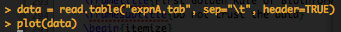
\includegraphics[width=\textwidth]{images/ex1_screenshot_c} \\
        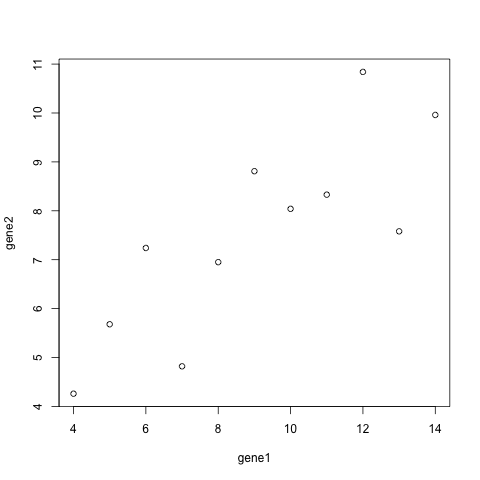
\includegraphics[width=\textwidth]{images/ex1_screenshot_d}        
      \end{column}
    \end{columns}
    \end{center}
  \end{frame}

  \begin{frame}
    \frametitle{Exercise 1}
    \framesubtitle{Always Plot the Data}
    \begin{center}
      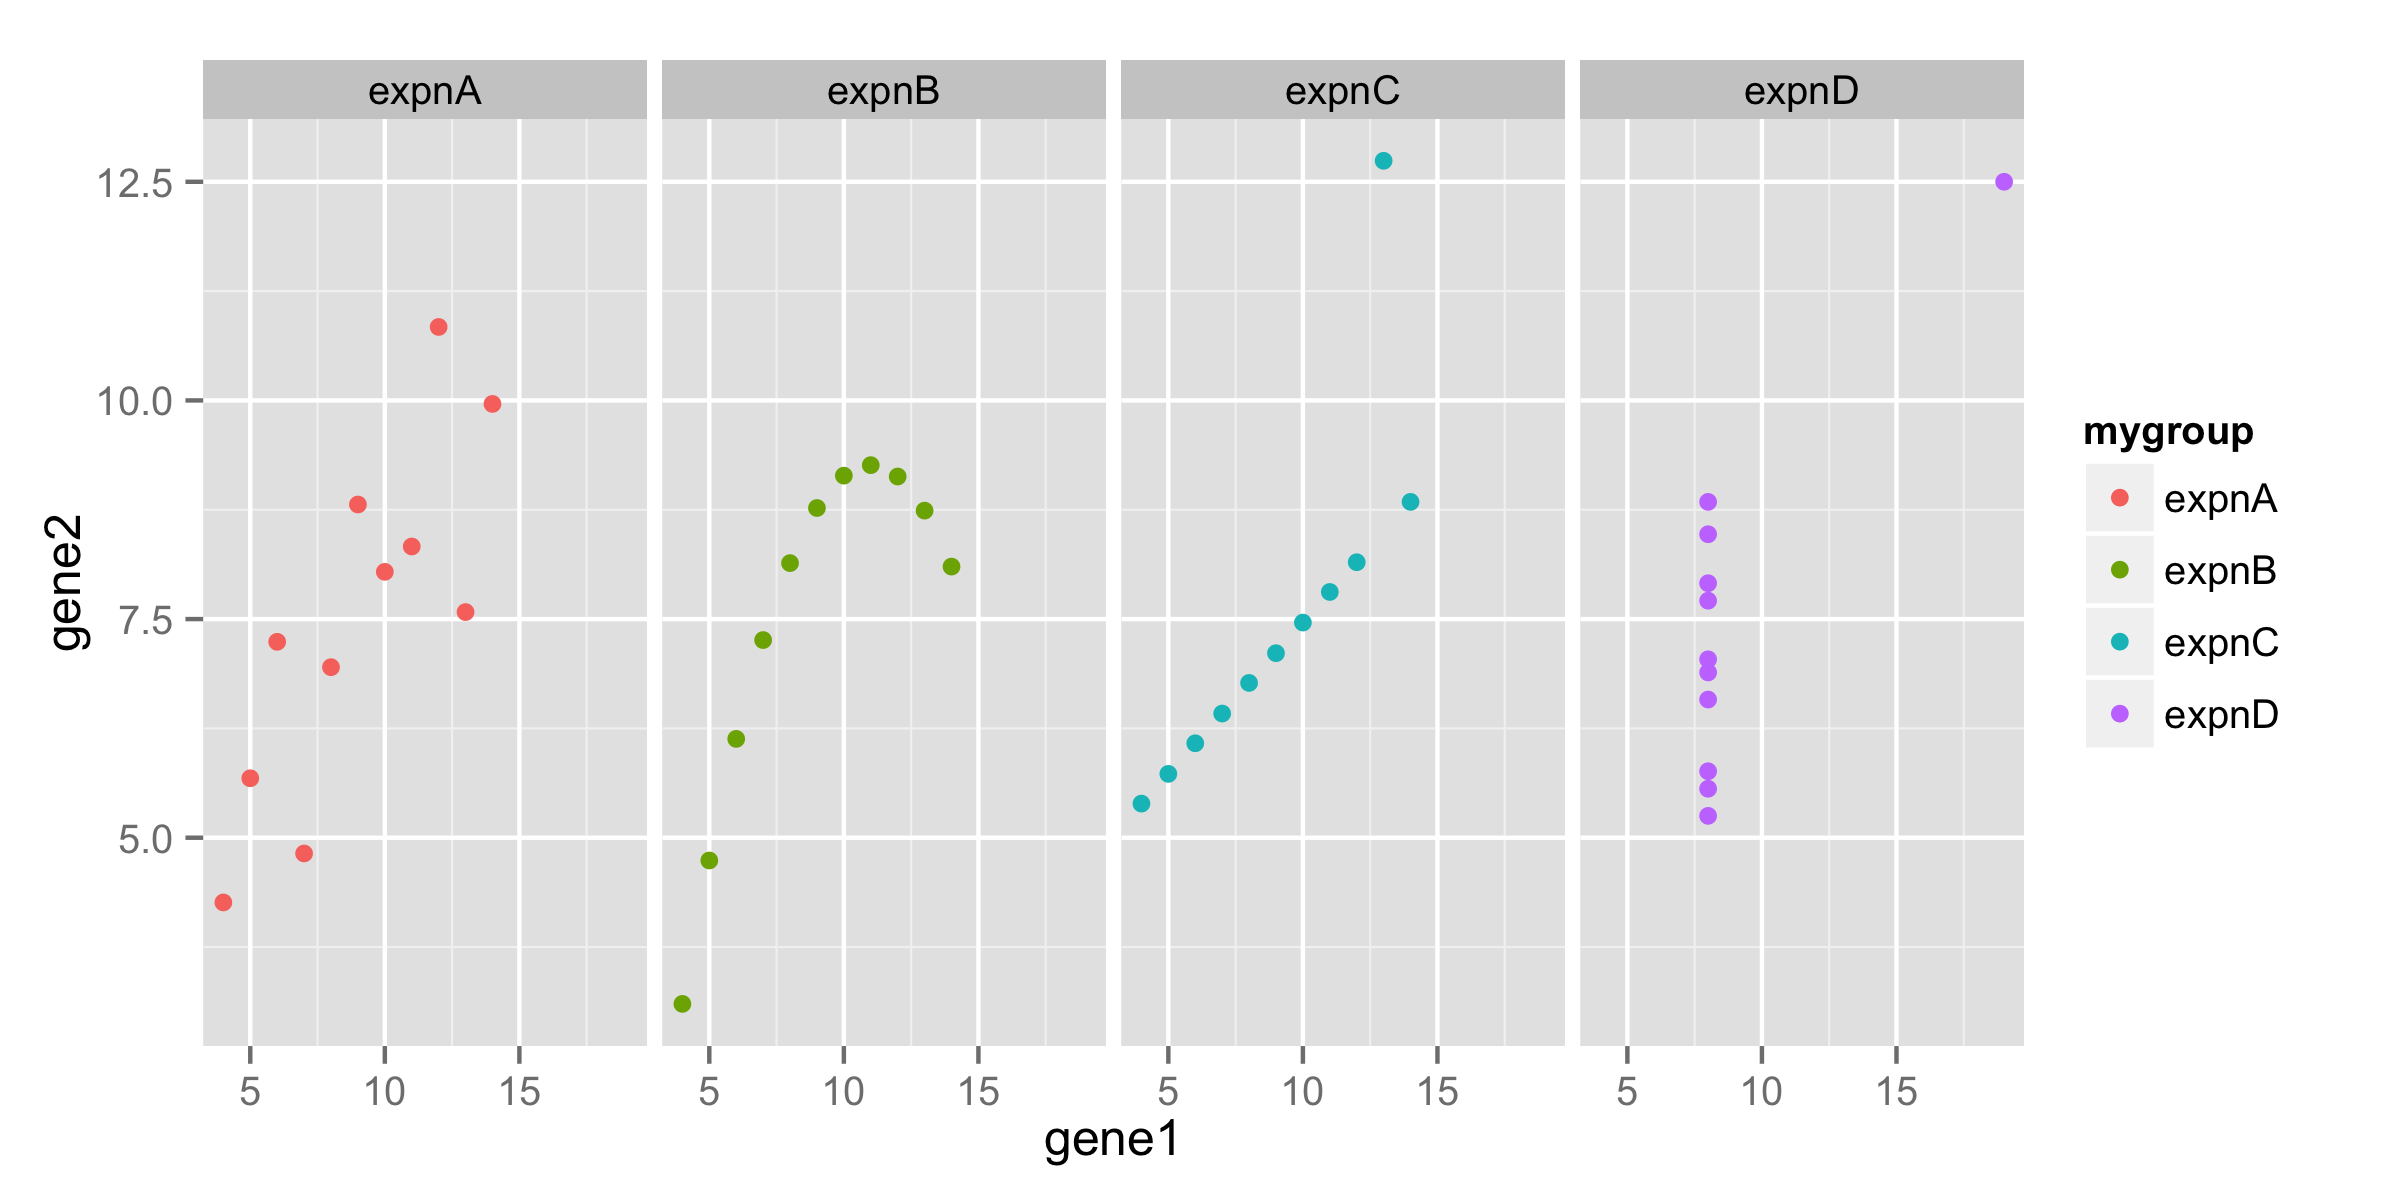
\includegraphics[width=\textwidth]{images/ex1_rplot} \\
    \end{center}
  \end{frame}

  \begin{frame}
    \frametitle{First Golden Rule of Bioinformatics}
    \framesubtitle{Do not trust the data}
	\begin{itemize}
	  \item Do not trust the data
	  \item Always inspect the raw data (trends, outliers, clustering)
	  \item Communicate with the data collectors! (don't be afraid of pedantry)
	  \begin{itemize}
	    \item Who? When? How?
	    \item You need to understand an experiment (easier if you helped design it) to analyse it
	    \item Be wary of block effects (experimenter, time, batch, etc.)
	  \end{itemize}
	\end{itemize}
  \end{frame}

  \subsection{Rule 2}
  \begin{frame}
    \frametitle{Exercise 2}
    \begin{itemize}
      \item You are in group A, B, C or D - this decides your database\\
      \texttt{dbA.tab}, \texttt{dbB.tab}, \texttt{dbC.tab}, \texttt{dbD.tab}
      \item You will use \texttt{BLAST} at the command-line to analyse your data
    \end{itemize}
  \end{frame}

  \begin{frame}
    \frametitle{Second Golden Rule of Bioinformatics}
    \framesubtitle{Do not trust the software}
	\begin{itemize}
	  \item Do not trust the software
	  \item You must understand the analysis/algorithm
	  \item Always sanity test
	  \item Test output for robustness to parameter choice
	  \item Software has bugs
	  \item Algorithms have assumptions, conditions, and applicable domains
	\end{itemize}
  \end{frame}
  
  \begin{frame}
    \frametitle{Exercise 3}
    \framesubtitle{Classification}
    \begin{itemize}
      \item Rule: If there is a vowel on one side of the card, there \textit{must} be an even number on the other side.
      \item Which cards \textit{must} be turned over to determine if the rule holds true? (How many, and which ones)
    \end{itemize}
    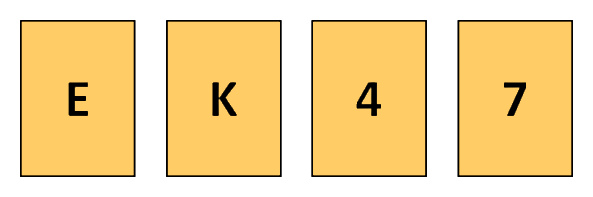
\includegraphics[width=\textwidth]{images/wason}
  \end{frame}

  \begin{frame}
    \frametitle{Exercise 3}
    \framesubtitle{Classification}
    \begin{itemize}
      \item This is equivalent to protein functional classification
      \item Rule: If there is a CRN/RxLR/T3SS domain, the protein \textit{must} be an effector.
    \end{itemize}
    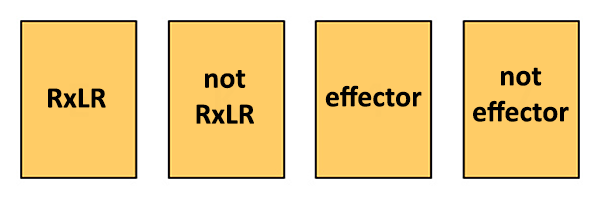
\includegraphics[width=\textwidth]{images/wason_rxlr}
  \end{frame}

  \begin{frame}
    \frametitle{Exercise 3}
    \framesubtitle{Classification}
    \begin{itemize}
      \item<1-> If you chose \emph{E} and \emph{4}
      \begin{itemize}
        \item<2-> You are in the typical majority group
        \item<3-> You are not correct
        \item<4-> You have been a victim of confirmation bias (System 1 thinking)
      \end{itemize}
      \item<5-> If you chose \emph{E} and \emph{7}
      \begin{itemize}
        \item<6-> Congratulations!
        \item<6-> Your choice was capable of \textit{falsifying} the rule.
      \end{itemize}
    \end{itemize}
  \end{frame}

  \begin{frame}
    \frametitle{Exercise 3}
    \framesubtitle{Classification}
    \begin{center}
	\begin{tabular}{c|c|c}
	  Card & Outcome & Rule \\
	  \hline
	  \hline
	    \multirow{2}{*}{E} & Even & True \emph{for this card} \\
	                                & Odd & \emph{violated} \\
	  \hline
	    \multirow{2}{*}{K} & Even & na \\
	                                & Odd & na \\	    
	  \hline
	    \multirow{2}{*}{4} & Vowel & True \emph{for this card} \\
	                                & Consonant & na \\
	  \hline
	    \multirow{2}{*}{7} & Vowel & \emph{violated} \\
	                                & Consonant & na \\	    
	\end{tabular}
    \end{center}
  \end{frame}

  \begin{frame}
    \frametitle{Third Golden Rule of Bioinformatics}
    \framesubtitle{Don't trust yourself}
	\begin{itemize}
	  \item Everyone has expectations of their data/experiment
	    \begin{itemize}
	      \item Beware cognitive errors, such as confirmation bias!
	      \item System 1 vs. System 2 $\approx$ reason vs. intuition
	    \end{itemize}
	  \item Think statistically! 
	    \begin{itemize}
	      \item Large datasets can be counterintuitive.
	      \item Always account for multiple tests.
	    \end{itemize}
	  \item Use test-driven development of analyses and code
	    \begin{itemize}
	      \item Use examples that pass \textit{and} fail
	    \end{itemize}	  
	\end{itemize}
  \end{frame}

  \subsection{Rule 3}
  \begin{frame}
    \frametitle{Third Golden Rule of Bioinformatics}
    \framesubtitle{Keep raw data and analysis separate}
	\begin{itemize}
	  \item Keep raw data and analysis separate
	  \item Avoid Excel! (off-by-one/copy errors/risk of changing data)
	  \item Make raw data read-only, and back it up immediately
	\end{itemize}
  \end{frame}


%%%
% SECTION: BLAST Essentials
  \section{BLAST Essentials}
  
    \begin{frame}
     \frametitle{How BLAST works}
    \end{frame}
   
    \begin{frame}
     \frametitle{Which BLAST tool should I use?}
    \end{frame}
     
    \begin{frame}
     \frametitle{Interpreting BLAST output}
    \end{frame}


%%%
% SECTION: 
  \section{}

  \begin{frame}
    \frametitle{Assessing Performance}
    \framesubtitle{Contingency Tables}
    \begin{center}
	\begin{tabular}{cc|c|c|}
	  \cline{3-4}
		& & \multicolumn{2}{|c|}{Condition (Gold standard)}\\
	  \cline{3-4}
		& & True & False \\
	  \hline
	  \multicolumn{1}{ |c| }{\multirow{2}{*}{Test outcome}}& 
	  \multicolumn{1}{ |c| }{Positive} & True Positive \cellcolor{green} & 
	    False Positive\cellcolor{red}\\
	  \cline{2-4}
	  \multicolumn{1}{ |c| }{} & \multicolumn{1}{ |c| }{Negative} & 
	    False Negative\cellcolor{red} & True Negative \cellcolor{green}\\
	  \hline
	\end{tabular}
	\end{center}
  \end{frame}

  \begin{frame}
  \end{frame}

% etc
\end{document}